\begin{frame}[fragile]{Visualização de um grafo simples completo, com um subgrafo $S$ em azul}

    \begin{figure}
        \centering

        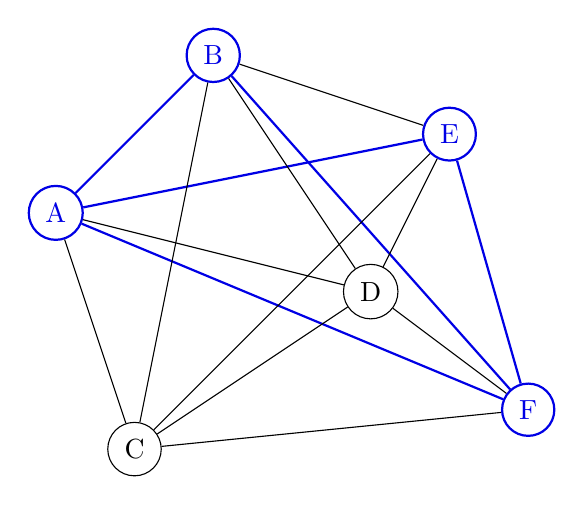
\begin{tikzpicture}
            \node[thick,blue!90!black,draw,circle] (A) at (0, 3) { A };
            \node[thick,blue!90!black,draw,circle] (B) at (2, 5) { B };
            \node[draw,circle] (C) at (1, 0) { C };
            \node[draw,circle] (D) at (4, 2) { D };
            \node[thick,blue!90!black,draw,circle] (E) at (5, 4) { E };
            \node[thick,blue!90!black,draw,circle] (F) at (6, 0.5) { F };

            \draw[thick,blue!90!black] (A) -- (B);
            \draw (A) -- (C);
            \draw (A) -- (D);
            \draw[thick,blue!90!black] (A) -- (E);
            \draw[thick,blue!90!black] (A) -- (F);
            \draw (B) -- (C);
            \draw (B) -- (D);
            \draw (B) -- (E);
            \draw[thick,blue!90!black] (B) -- (F);
            \draw (C) -- (D);
            \draw (C) -- (E);
            \draw (C) -- (F);
            \draw (D) -- (E);
            \draw (D) -- (F);
            \draw[thick,blue!90!black] (E) -- (F);
        \end{tikzpicture}

    \end{figure}

\end{frame}
